\documentclass[a4paper]{article}

\usepackage[UTF8]{ctex}
\usepackage{graphicx}
\usepackage{xurl}
\usepackage{cite}
\usepackage{hyperref}
\hypersetup{
    colorlinks=true,
    allcolors=black,
    breaklinks=true
}

\begin{document}

\songti

\title{电力电子技术基础第一次作业}
\author{2018040401018 李金豪}

\maketitle

\section{Question 1}

题目:从未知的诞生的电力电子技术

摘要:电力电子技术是由电气工程主要的三门学科(电子学、电力学和控制理论)交叉而成的技术。然后这项技术的重大意义并没有被广泛的认知。并且这项技术领域的专家一直局限于通信层面以及合作解决有挑战性的问题。这篇文章宣告了这种现状的终结,引领这门全新的、重要的学科——电力电子技术的发展

\begin{figure}[htbp]
    \centering
    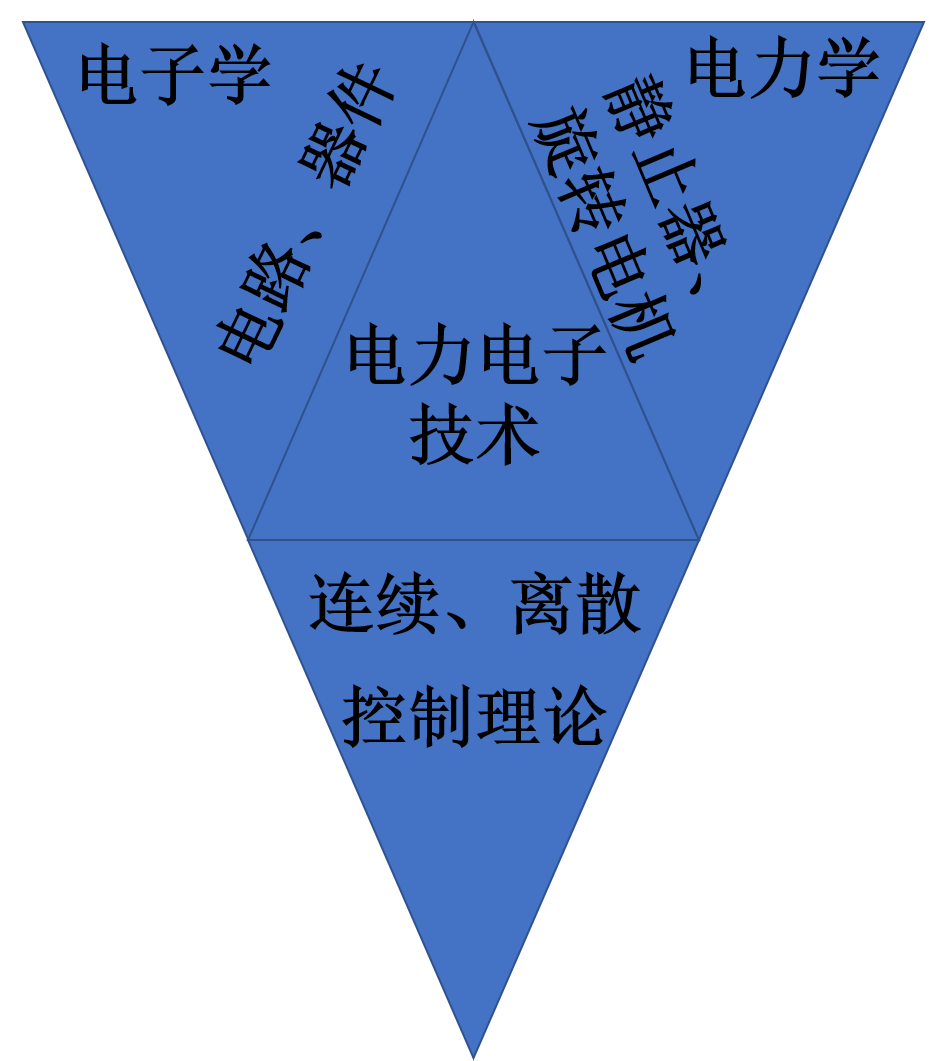
\includegraphics[width=4cm,height=5cm]{pic.png}
    \caption{倒三角形}
\end{figure}


\section{Question 2}

1. 发电环节 \cite{ref1}

发电环节使用最为广泛的是静止励磁系统,电力电子技术的发展取代了以往的励磁环节,实现了静止励磁操作,使得电力控制趋于简单化,大幅度降低了电能成本,并且提高了整个电力系统的工作效率 

2. 输电环节 

传统电力输送会在传输过程中产生电能损耗。应用FACTS(柔性交流输电技术),可以控制电力输送时的参数,合理分配输电功率,降低输电时电能损耗,从而降低输电成本

此外,HVDC(高压直流输电技术)使用的即为电子电力器件——晶闸管,它使得高压直流输电表现良好,降低了高压直流输电的电能损耗

3. 配电环节

在配电环节应用电力电子技术可以提高配电质量。具体应用为用户电力技术和FACTS技术。其中FACTS技术能够控制电路中的电流和电压,从而提升配电质量。用户电力技术能够快速解决配电系统中出现的重大问题,提高了配电系统的稳定性和安全性

4. 用电环节

家用LED灯、变频空调等家用电器均用到电力电子器件及相关技术,可以降低电器的能耗,节能减排

\section{Question 3}

1. 在电力驱动主模块的应用 \cite{ref2}

在直流电机驱动系统中应用的是DC-DC转换器,即直流斩波器。两象限直流斩波器能把蓄电池的直流电压转换为可变的直流电压,用于直流电动机的驱动。早期应用较广泛的是晶闸管斩波调速,通过均匀改变直流电动机的端电压,控制电动机的电流,来实现电动机的无级调速。随着电子电力期间的不断发展,它逐渐被其它电力晶体管(如GTO,MOSFET,BTR及IGBT等)斩波调速装置所取代

在异步电机驱动系统中,由于蓄电池以直流电形式输出能量,若要用蓄电池输出的能量驱动交流电机,要先将直流电逆变为交流电,应用的电子电力器件是DC-AC转换器,即逆变器,它将蓄电池的直流电转换为频率和电压都可调的交流电。通常采用的是SPWM逆变器。

2. 在其它模块的应用

在车载电源模块中的充电控制器需要电网电源的输出的交流电转换为相应电压的直流电,并在充电过程中按照要求控制其电流的大小,需要用到电力电子技术

在电动汽车辅助系统中,辅助动力源中包含DC-DC功率转换器件,将蓄电池电源输出的直流电转换为供给电动汽车其它各种辅助装置所需要的电能

\begin{thebibliography}{99}
    \bibitem{ref1} \url{https://wenku.baidu.com/view/303368000d22590102020740be1e650e52eacfa6.html}
    \bibitem{ref2} 张剑.电力电子技术在电动汽车中的应用分析[J].电子世界,2017(02):162-163
\end{thebibliography}

\end{document}